% =====================================================================
%  SLR_tallos_aguacate_v1 — versión LaTeX
%  Compilar con XeLaTeX o LuaLaTeX (en Overleaf: Menu > Compiler > XeLaTeX).
%  Fuente: Calibri (si no está instalada se usa Carlito, métricamente igual).
% =====================================================================
\documentclass[11pt]{article}

% --- Página: carta, márgenes 3 cm (izq./der.) y 2,5 cm (sup./inf.) ---
\usepackage[letterpaper,left=3cm,right=3cm,top=2.5cm,bottom=2.5cm]{geometry}

% --- Idioma y fuente ---
\usepackage{fontspec}
\IfFontExistsTF{Calibri}{\setmainfont{Calibri}}{%
  \setmainfont{Carlito}[Extension=.ttf,UprightFont=*-Regular,BoldFont=*-Bold,
    ItalicFont=*-Italic,BoldItalicFont=*-BoldItalic]}
\usepackage[spanish,es-nolayout,es-noshorthands,es-nodecimaldot,es-nopercent]{babel}

% --- Paquetes ---
\usepackage{graphicx}
\usepackage[table]{xcolor}
\usepackage{array}
\usepackage{longtable}
\usepackage{enumitem}
\usepackage{titlesec}
\usepackage{caption}
\usepackage{xurl}
\urlstyle{same}
\usepackage{ragged2e}

% --- Párrafos: interlineado 1,08 y 8 pt después de cada párrafo (Word) ---
\linespread{1.08}
\setlength{\parindent}{0pt}
\setlength{\parskip}{8pt}
\newcommand{\sangria}{\hspace*{1.27cm}}
\pagestyle{empty}   % el documento original no tiene numeración de páginas
\emergencystretch=2em

% --- Encabezados ---
% "1.  Introducción": 12 pt, negrita, numerado
\titleformat{\section}{\fontsize{12}{14.5}\selectfont\bfseries}{\makebox[0.63cm][l]{\thesection.}}{0pt}{}
\titlespacing*{\section}{0pt}{12pt}{6pt}
% "2.1 Diseño de la revisión": 11 pt, negrita
\titleformat{\subsection}{\normalsize\bfseries}{\thesubsection}{0.3em}{}
\titlespacing*{\subsection}{0pt}{10pt}{5pt}

% --- Títulos de tablas y figuras: "Tabla 1." en negrita + título en cursiva (10 pt) ---
\captionsetup{font={small},labelfont=bf,textfont=it,labelsep=period,
  justification=raggedright,singlelinecheck=false}
\captionsetup[table]{name=Tabla,position=top,skip=4pt}
\captionsetup[figure]{name=Figura,position=bottom,skip=4pt}
\setlength{\LTcapwidth}{\linewidth}
\setlength{\LTpre}{8pt}
\setlength{\LTpost}{0pt}

% --- Tablas: margen interno de celda como en Word ---
\setlength{\tabcolsep}{0.123cm}
\renewcommand{\arraystretch}{1.15}

% --- Nota de tabla o figura (9 pt) ---
\newcommand{\nota}[1]{\par\vspace{-6pt}{\fontsize{9}{11}\selectfont\justifying #1\par}\vspace{2pt}}

% --- Viñetas (preguntas de investigación y limitaciones) ---
\setlist[itemize]{label=\textbullet,leftmargin=1.26cm,labelsep=0.4cm,
  itemsep=3pt,parsep=0pt,topsep=0pt}

% --- Referencias con sangría francesa de 1,27 cm ---
\newcommand{\referencia}[1]{{\RaggedRight\hangindent=1.27cm\hangafter=1 #1\par}\vspace{-2pt}}

\begin{document}
\justifying
\begingroup\setlength{\parskip}{0pt}

{\centering Prácticas preprofesionales – Departamento de Ciencias de la Computación\par}

{\centering \hangindent=0.635cm\hangafter=1 Universidad de las Fuerzas Armadas ESPE\par}

\noindent\hangindent=0.635cm\hangafter=1  \textbf{Autor/a: Ariel Llumiquinga}\par

\noindent\hangindent=0.635cm\hangafter=1  \textbf{Tutora: Ing. Doris Chicaiza}\par

\noindent\hangindent=0.635cm\hangafter=1  \textbf{Proyecto: Smart Agriculture}\par

\noindent\hangindent=0.635cm\hangafter=1  \textbf{Actividad del itinerario: 8. Redacción del borrador de la SLR (tareas T23–T26)}\par

\noindent\hangindent=0.635cm\hangafter=1  \textbf{Versión: 1 (borrador)}\par

\noindent\hangindent=0.635cm\hangafter=1  \textbf{Fecha: 2 de octubre de 2026.}\par

\noindent\hangindent=0.635cm\hangafter=1  \textbf{Estado: Borrador para revisión de la tutora.}\par

\endgroup

\vspace*{\baselineskip}

\vspace{6pt}

{\centering\fontsize{14}{17}\selectfont \textbf{Enfermedades del tallo del aguacate (}\textbf{\textit{Persea americana}}\textbf{) y sistemas basados en inteligencia artificial para su diagnóstico en el marco de la agricultura inteligente: revisión sistemática de la literatura}\par}

\vspace{2pt}

\section*{Resumen}

Las enfermedades del tallo, las ramas y el tronco comprometen la estructura y la productividad del aguacate, y su diagnóstico depende hoy del laboratorio. Esta revisión sistemática analizó la evidencia sobre esas enfermedades y sobre los sistemas basados en inteligencia artificial (IA) para diagnosticar enfermedades en cultivos, con el fin de fundamentar una aplicación móvil de diagnóstico en tallos de aguacate. Se siguieron las directrices de Kitchenham y Charters (como se citó en Martinelli et al., 2024) y el reporte se ajustó a la declaración PRISMA 2020. Dieciséis cadenas ejecutadas en Scopus, ScienceDirect y Springer Link exportaron 78 registros; tras retirar 14 duplicados y 9 revisiones, se cribaron 55, se evaluaron 22 a texto completo y se incluyeron 17 estudios (12 fitopatológicos y 5 tecnológicos); 1 quedó en reserva. Todos los estudios incluidos obtuvieron calidad alta. Botryosphaeriaceae fue el grupo de patógenos dominante, con \textit{Neofusicoccum parvum} como la especie más reportada, seguido de \textit{Colletotrichum}, \textit{Phytophthora} y \textit{Fusarium}; los estudios proceden de la cuenca mediterránea, Sudamérica y México, y ninguno de Ecuador. Los síntomas externos —cancros con exudado blanquecino, corteza oscura y agrietada, muerte descendente desde el ápice y lesiones desde el injerto— pueden fotografiarse, pero se superponen entre patógenos, y la necrosis interna avanza antes que la externa. Ningún estudio aplicó IA al tallo: los sistemas tecnológicos trabajan con hojas o frutos, procesan la imagen en un servidor, no funcionan sin conexión y solo uno evaluó formalmente a sus usuarios. Se recomienda una aplicación que clasifique tipos de síntoma del tallo, entrenada con imágenes propias de campo, con modelos ligeros ejecutados en el teléfono y evaluada con agricultores y técnicos.

\textbf{Palabras clave:} aguacate; enfermedades del tallo; Botryosphaeriaceae; aprendizaje profundo; aplicación móvil; interacción persona-ordenador; agricultura inteligente.

\section{Introducción}

Las plagas y enfermedades causan cerca del 30 \% de las pérdidas mundiales de cultivos, y su identificación tradicional depende de la experiencia humana, lo que la vuelve lenta, costosa y a menudo imprecisa (Majdalawieh et al., 2025). Los agricultores vigilan las plantas de forma manual y a simple vista (Sajitha et al., 2024), y la inspección visual depende de la pericia de cada persona (Odounfa et al., 2024). La agricultura de precisión y el aprendizaje profundo ofrecen una alternativa: las redes neuronales convolucionales (CNN) son el enfoque más usado para reconocer enfermedades en imágenes (Majdalawieh et al., 2025), y su ejecución en teléfonos permite el diagnóstico en el propio campo, incluso sin conexión (Saini et al., 2026).

\sangria El aguacate es un cultivo de gran importancia económica, y las mismas condiciones cálidas que lo favorecen promueven a los hongos de la familia Botryosphaeriaceae, causantes de cancros en ramas, muerte descendente y pudriciones del fruto (Möller et al., 2025). El diagnóstico de estas enfermedades se basa en los síntomas observados en campo (Silva et al., 2025) y su confirmación requiere aislamiento e identificación molecular, un proceso que puede tardar semanas (Möller et al., 2025). A la vez, los modelos de IA que superan el 98 \% de exactitud con imágenes de laboratorio bajan al 70–80 \% en campo (Saini et al., 2026), y la falta de interpretabilidad limita la confianza de los agricultores (Lin et al., 2026), por lo que una aplicación útil necesita tanto un buen modelo como un diseño centrado en el usuario (Martinelli et al., 2024).

\sangria Las revisiones disponibles abordan estos temas por separado. Las tecnológicas analizan la IA para enfermedades de cultivos en general (Lin et al., 2026; Majdalawieh et al., 2025; Munjal et al., 2023; Odounfa et al., 2024; Saini et al., 2026; Sajitha et al., 2024) y señalan que la detección en tallos, flores y frutos casi no se ha estudiado (Sajitha et al., 2024); la fitopatológica describe las Botryosphaeriaceae del aguacate sin tratar su diagnóstico automatizado (Möller et al., 2025). El proyecto Smart Agriculture, cuyo objetivo es una aplicación móvil para diagnosticar enfermedades y alteraciones visibles en el tallo del aguacate, necesita ambos conocimientos.

\sangria Por ello, esta revisión tiene como objetivo analizar y sintetizar la literatura sobre las enfermedades y alteraciones del tallo del aguacate —sus agentes causales, síntomas visibles y métodos de detección— y sobre los sistemas basados en IA y visión por computador para diagnosticar enfermedades en cultivos —sus técnicas, datos, métricas, implementación e interacción persona-ordenador (IPO)—, a fin de identificar buenas prácticas y brechas para la aplicación del proyecto. Las preguntas de investigación son:

\begin{itemize}

  \item \textbf{RQ1.} ¿Qué agentes causales y enfermedades afectan al tallo, las ramas y el tronco del aguacate, y en qué regiones se han reportado?

  \item \textbf{RQ2.} ¿Qué síntomas visibles producen estas enfermedades y qué métodos se utilizan para su detección y diagnóstico?

  \item \textbf{RQ3.} ¿Qué técnicas de IA y visión por computador, conjuntos de datos y métricas emplean los sistemas de diagnóstico de enfermedades en cultivos?

  \item \textbf{RQ4.} ¿Qué características de implementación (plataforma, inferencia, funcionamiento sin conexión) y de IPO presentan estos sistemas?

  \item \textbf{RQ5.} ¿Qué brechas y oportunidades se identifican para una aplicación móvil de diagnóstico de enfermedades en tallos de aguacate?

\end{itemize}

\sangria El documento se organiza en metodología (sección 2), resultados por pregunta (sección 3), discusión, con las brechas y las limitaciones (sección 4), y conclusiones (sección 5).

\section{Metodología}

\subsection{Diseño de la revisión}

La revisión siguió las directrices de Kitchenham y Charters para revisiones sistemáticas (como se citó en Martinelli et al., 2024) y se reporta conforme a la declaración PRISMA 2020, aplicada en revisiones del área (Lin et al., 2026; Majdalawieh et al., 2025; Odounfa et al., 2024; Sajitha et al., 2024). El protocolo (versión 3, 1 de octubre de 2026) define una sola revisión y un solo diagrama de flujo con dos categorías de estudios primarios: \textbf{fitopatológicos}, sobre las enfermedades del tallo del aguacate (identificadores A0001–A0048), y \textbf{tecnológicos}, sobre sistemas de IA para diagnosticar enfermedades en cultivos (T0001–T0020). Cada categoría tiene sus propios criterios de elegibilidad y de calidad. Todo el proceso se registró en una matriz de Excel (versión 5), que calcula los conteos por fórmula.

\subsection{Fuentes de información y estrategia de búsqueda}

Se consultaron Scopus, ScienceDirect y Springer Link, bases con acceso institucional; IEEE Xplore y Web of Science no se consultaron por falta de acceso. Las búsquedas se aplicaron a título, resumen y palabras clave, con filtros de 2003 a 2026 (fitopatológicas) y de 2015 a 2026 (tecnológicas), en español o inglés; los filtros de las cadenas complementarias no se registraron. Se ejecutaron 16 cadenas en tres momentos (Tabla 1; texto exacto en el Anexo A). Las cadenas complementarias de ScienceDirect son más cortas porque esta base limita a ocho los operadores booleanos por campo (Yuan et al., 2026); se usaron para recuperar revisiones que sirven como antecedentes. Los totales de resultados (hits) de cada base no se registraron al buscar, por lo que la identificación parte de los registros exportados.

{\fontsize{9}{11}\selectfont
\begin{longtable}{|>{\RaggedRight\arraybackslash}p{3.810cm}|>{\RaggedRight\arraybackslash}p{3.104cm}|>{\RaggedRight\arraybackslash}p{2.399cm}|>{\RaggedRight\arraybackslash}p{3.171cm}|>{\RaggedRight\arraybackslash}p{1.870cm}|}
\caption{Cadenas de búsqueda ejecutadas por grupo y base de datos}\\
\hline
\rowcolor[HTML]{D9E2F3}
\multicolumn{1}{|>{\centering\arraybackslash}m{3.810cm}|}{\textbf{Grupo}} & \multicolumn{1}{>{\centering\arraybackslash}m{3.104cm}|}{\textbf{Base de datos}} & \multicolumn{1}{>{\centering\arraybackslash}m{2.399cm}|}{\textbf{N.º de cadena}} & \multicolumn{1}{>{\centering\arraybackslash}m{3.171cm}|}{\textbf{Fecha}} & \multicolumn{1}{>{\centering\arraybackslash}m{1.870cm}|}{\textbf{Registros exportados}} \\ \hline
\endfirsthead
\hline
\rowcolor[HTML]{D9E2F3}
\multicolumn{1}{|>{\centering\arraybackslash}m{3.810cm}|}{\textbf{Grupo}} & \multicolumn{1}{>{\centering\arraybackslash}m{3.104cm}|}{\textbf{Base de datos}} & \multicolumn{1}{>{\centering\arraybackslash}m{2.399cm}|}{\textbf{N.º de cadena}} & \multicolumn{1}{>{\centering\arraybackslash}m{3.171cm}|}{\textbf{Fecha}} & \multicolumn{1}{>{\centering\arraybackslash}m{1.870cm}|}{\textbf{Registros exportados}} \\ \hline
\endhead
\textbf{Fitopatológicas} & Scopus & 1, 4, 5, 6, 7, 8, 9 & 17/09/2026, 18/09/2026 & 46 \\ \hline
\textbf{Fitopatológicas} & Science Direct & 2 & 18/09/2026 & 7 \\ \hline
\textbf{Fitopatológicas} & Springer Link & 3 & 17/09/2026 & 3 \\ \hline
\textbf{Tecnológicas} & Scopus & 12, 13, 14 & 25/09/2026 & 13 \\ \hline
\textbf{Tecnológicas} & Springer Link & 15 & 25/09/2026 & 1 \\ \hline
\textbf{Complementarias (revisiones)} & Science Direct & 16, 17, 18 & 01/10/2026 & 8 \\ \hline
\rowcolor[HTML]{FFF2CC}
\textbf{Total} & Scopus, ScienceDirect, Springer Link & 16 cadenas & 17/09/2026 – 01/10/2026 & 78 \\ \hline
\end{longtable}}

\nota{\textit{Nota.} Elaboración propia a partir de la hoja Cadenas\_de\_busqueda de la matriz. Las cadenas 13 y 14 se exportaron junto con la 12; los números 10 y 11 no se usaron.}

\subsection{Criterios de elegibilidad}

Los criterios se definieron por categoría (Tabla 2). Las revisiones se identificaron y se retiraron antes del cribado ("otros motivos"), y se utilizaron como fuentes de los antecedentes.

{\fontsize{9}{11}\selectfont
\begin{longtable}{|>{\RaggedRight\arraybackslash}p{2.399cm}|>{\RaggedRight\arraybackslash}p{6.225cm}|>{\RaggedRight\arraybackslash}p{6.225cm}|}
\caption{Criterios de inclusión y exclusión por categoría}\\
\hline
\rowcolor[HTML]{D9E2F3}
\multicolumn{1}{|>{\centering\arraybackslash}m{2.399cm}|}{\textbf{Categoría}} & \multicolumn{1}{>{\centering\arraybackslash}m{6.225cm}|}{\textbf{Criterios de inclusión}} & \multicolumn{1}{>{\centering\arraybackslash}m{6.225cm}|}{\textbf{Criterios de exclusión}} \\ \hline
\endfirsthead
\hline
\rowcolor[HTML]{D9E2F3}
\multicolumn{1}{|>{\centering\arraybackslash}m{2.399cm}|}{\textbf{Categoría}} & \multicolumn{1}{>{\centering\arraybackslash}m{6.225cm}|}{\textbf{Criterios de inclusión}} & \multicolumn{1}{>{\centering\arraybackslash}m{6.225cm}|}{\textbf{Criterios de exclusión}} \\ \hline
\endhead
\textbf{Fitopatológica} & \textbf{CI-F1.} Trata sobre aguacate.\newline \textbf{CI-F2.} Menciona Phytophthora, Lasiodiplodia, Botryosphaeriaceae, Colletotrichum, Fusarium o Nectria/Rugonectria.\newline \textbf{CI-F3.} Aporta información del tallo, las ramas o el tronco.\newline \textbf{CI-F4.} Estudio primario, en español o inglés, de 2003 a 2026. & \textbf{CE-F1.} Solo raíz, hoja o fruto (incluye la pudrición peduncular, que es del fruto).\newline \textbf{CE-F2.} Revisión.\newline \textbf{CE-F3.} Sin especie ni órgano.\newline \textbf{CE-F4.} Duplicado.\newline \textbf{CE-F5.} Fuera de periodo o idioma. \\ \hline
\textbf{Tecnológica} & \textbf{CI-T1.} Detección o diagnóstico de enfermedades de plantas.\newline \textbf{CI-T2.} Usa IA, aprendizaje automático o profundo, o visión por computador.\newline \textbf{CI-T3.} Relacionado con una app, un dispositivo o un sistema de apoyo, o analiza su viabilidad.\newline \textbf{CI-T4.} Estudio primario, en español o inglés, de 2015 a 2026. & \textbf{CE-T1.} No usa IA.\newline \textbf{CE-T2.} No trata enfermedades (madurez, calidad, estrés hídrico).\newline \textbf{CE-T3.} Revisión.\newline \textbf{CE-T4.} Duplicado, fuera de periodo o idioma. \\ \hline
\end{longtable}}

\nota{\textit{Nota.} Elaboración propia a partir de el protocolo v3.}

\subsection{Gestión de registros y selección de estudios}

Los 78 registros exportados se consolidaron con un identificador único. Se eliminaron 10 duplicados dentro de una misma base y 4 duplicados entre bases (mismo DOI; se conservó el registro de Scopus), y se retiraron 9 revisiones. Los 55 registros restantes se cribaron por título, resumen y palabras clave; los casos cuyo resumen dejaba ambiguo el órgano estudiado pasaron a texto completo, y la decisión a texto completo se tomó leyendo el PDF. La selección la realizó un revisor principal (el autor). Según el protocolo, la tutora verifica los cinco casos dudosos (A0029, A0031, A0035, A0042 y T0012) y una muestra del 10 \% de los excluidos en el cribado (A0010, A0011, A0034 y T0008), obtenida por sorteo con semilla fija.

\subsection{Evaluación de la calidad}

Los estudios elegibles se evaluaron con diez criterios por categoría (Tabla 3), puntuados con 0 (no cumple), 1 (parcial) o 2 (cumple), para un total de 0 a 20: calidad alta (16–20), media (11–15) o baja (≤ 10). Las reglas operativas de cada puntaje quedaron escritas en la matriz para su verificación. Se prestó atención al tamaño de la muestra y a los postulados de Koch en los estudios fitopatológicos, y al uso de datos de laboratorio, la validación en campo y la evaluación con usuarios en los tecnológicos.

{\fontsize{9}{11}\selectfont
\begin{longtable}{|>{\RaggedRight\arraybackslash}p{1.517cm}|>{\RaggedRight\arraybackslash}p{6.666cm}|>{\RaggedRight\arraybackslash}p{6.666cm}|}
\caption{Criterios de calidad Q1–Q10 por categoría}\\
\hline
\rowcolor[HTML]{D9E2F3}
\multicolumn{1}{|>{\centering\arraybackslash}m{1.517cm}|}{\textbf{Código}} & \multicolumn{1}{>{\centering\arraybackslash}m{6.666cm}|}{\textbf{Estudios fitopatológicos}} & \multicolumn{1}{>{\centering\arraybackslash}m{6.666cm}|}{\textbf{Estudios tecnológicos}} \\ \hline
\endfirsthead
\hline
\rowcolor[HTML]{D9E2F3}
\multicolumn{1}{|>{\centering\arraybackslash}m{1.517cm}|}{\textbf{Código}} & \multicolumn{1}{>{\centering\arraybackslash}m{6.666cm}|}{\textbf{Estudios fitopatológicos}} & \multicolumn{1}{>{\centering\arraybackslash}m{6.666cm}|}{\textbf{Estudios tecnológicos}} \\ \hline
\endhead
\textbf{Q1} & Objetivo claro & Objetivo claro \\ \hline
\textbf{Q2} & Patógeno identificado & Problema de detección definido \\ \hline
\textbf{Q3} & Síntomas en el tallo descritos & Dataset especificado \\ \hline
\textbf{Q4} & Estudio en aguacate & Modelo replicable \\ \hline
\textbf{Q5} & Metodología replicable & Métricas con validación adecuada \\ \hline
\textbf{Q6} & Evidencia (imágenes, mediciones, secuencias) & Comparación con otros modelos \\ \hline
\textbf{Q7} & Métodos de detección útiles para la app & Implementación en app o dispositivo \\ \hline
\textbf{Q8} & Contexto geográfico & IPO, UX o usabilidad \\ \hline
\textbf{Q9} & Resultados coherentes & Resultados coherentes y reproducibles \\ \hline
\textbf{Q10} & Fuente confiable y actual & Fuente confiable y actual \\ \hline
\end{longtable}}

\nota{\textit{Nota.} Elaboración propia a partir de el protocolo v3.}

\subsection{Extracción y síntesis}

De cada estudio elegible se extrajeron el tipo de estudio, el aporte principal, el país y, según la categoría, el grupo de patógeno, las especies, el órgano, los síntomas en el tallo y el método de detección, o bien el modelo, el conjunto de datos, las métricas, la plataforma, el tipo de inferencia y los aspectos de IPO. Además de la calidad, se valoró la alineación con el objetivo (alta, media o baja). Un estudio se incluyó en la síntesis si su calidad y su alineación eran altas o medias; en caso contrario quedó en reserva (se cita, pero no entra en la síntesis). La síntesis es narrativa y está organizada por pregunta de investigación, con tablas comparativas.

\section{Resultados}

\subsection{Selección de los estudios}

La Figura 1 resume el proceso. De 78 registros identificados (Scopus 59, ScienceDirect 15 y Springer Link 4) se eliminaron 14 duplicados y 9 revisiones. En el cribado se excluyeron 33 de 55 registros: 13 por tratar solo del fruto, 12 solo de la raíz, 2 sin información del tallo, 5 por no abordar enfermedades y 1 por no usar IA. Los 22 informes restantes se recuperaron completos; a texto completo se excluyeron 4 (Anexo B) y 1 quedó en reserva por su baja alineación: el anuncio de genoma de Rincón López et al. (2026) [A0017], que no describe síntomas. Se incluyeron 17 estudios: 12 fitopatológicos y 5 tecnológicos.

\begin{center}

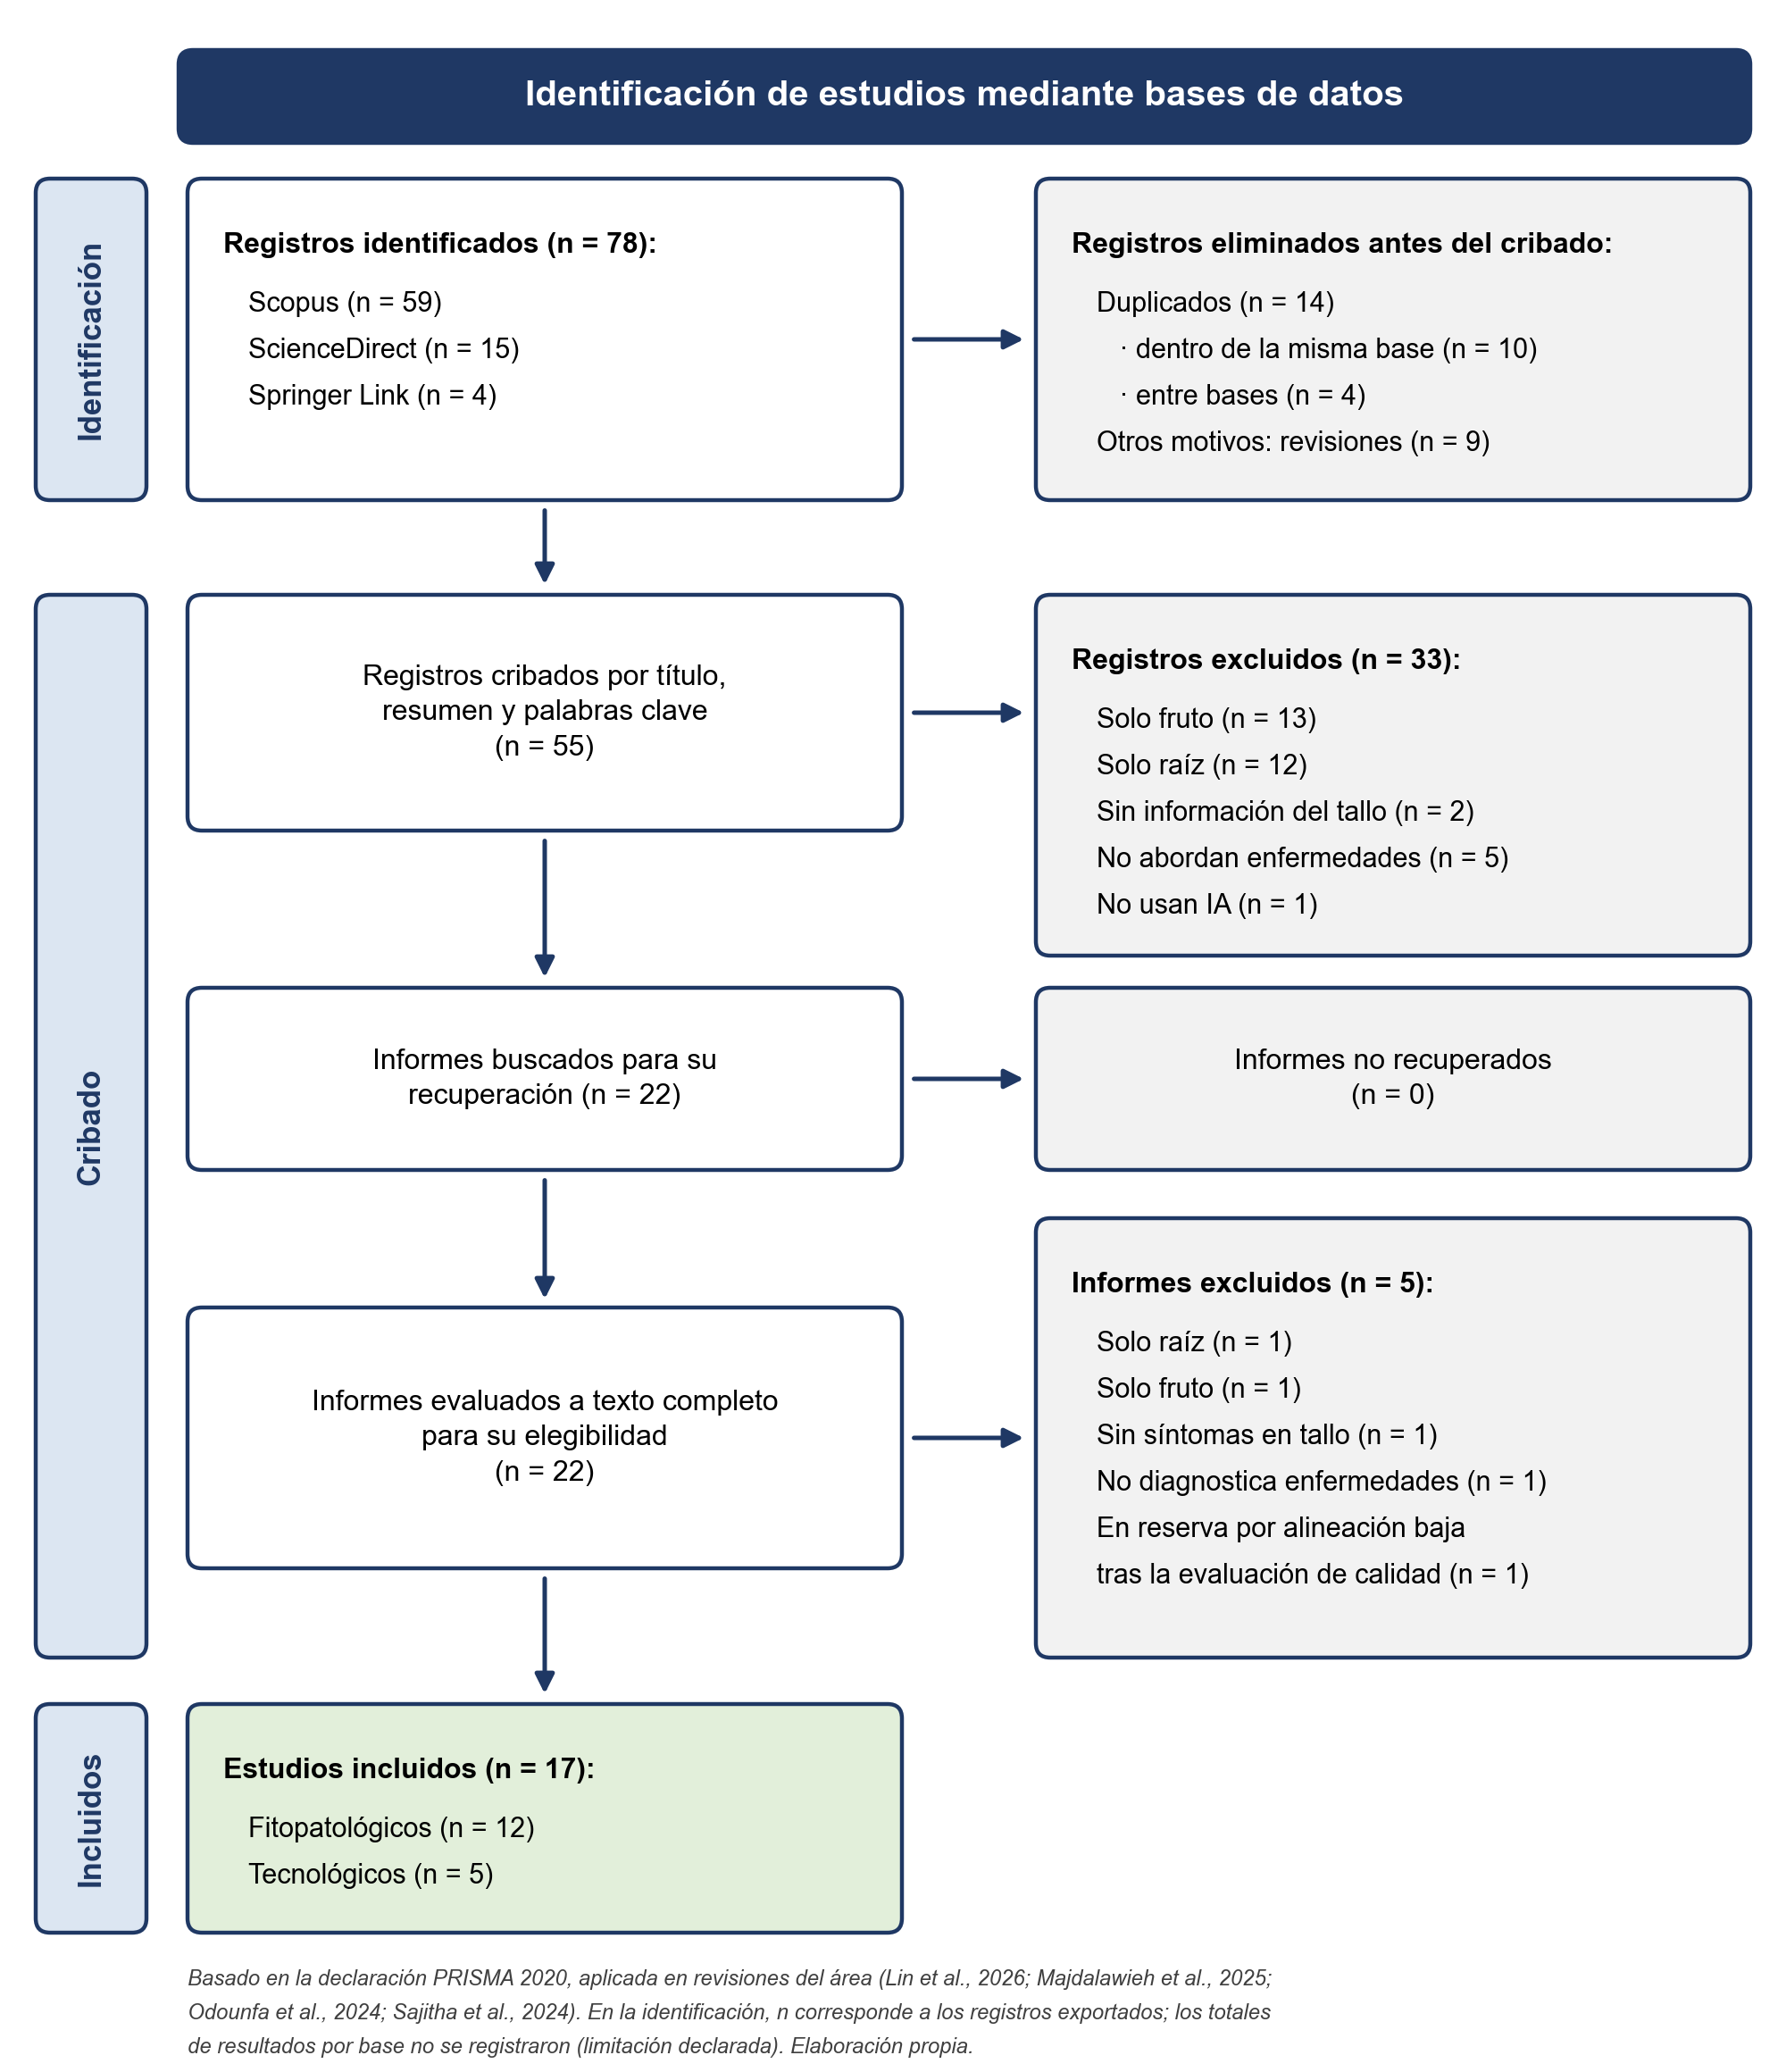
\includegraphics[width=14.224cm]{figuras/Figura1_PRISMA_2020.png}

\captionof{figure}{Diagrama de flujo PRISMA 2020 de la selección de estudios}

\end{center}

\nota{\textit{Nota.} Elaboración propia a partir de la hoja PRISMA de la matriz; diagrama basado en la declaración PRISMA 2020, aplicada en revisiones del área (Lin et al., 2026; Majdalawieh et al., 2025; Odounfa et al., 2024; Sajitha et al., 2024).}

\subsection{Características y calidad de los estudios}

Los estudios fitopatológicos incluidos son recientes (8 de 12 publicados entre 2024 y 2026; el más antiguo es de 2019) y proceden sobre todo de la cuenca mediterránea —España, Italia y Turquía— y, en menor medida, de Sudamérica (Brasil, Perú y Chile) y México. Ninguno se realizó en Ecuador. Los tecnológicos provienen de India, Pakistán, Perú, Grecia y España. La calidad fue alta en todos los incluidos (Tabla 4); el estudio en reserva obtuvo calidad media. Los puntajes detallados por criterio se presentan en el Anexo C.

{\fontsize{8.5}{10.4}\selectfont
\begin{longtable}{|>{\RaggedRight\arraybackslash}p{4.163cm}|>{\RaggedRight\arraybackslash}p{2.046cm}|>{\RaggedRight\arraybackslash}p{3.171cm}|>{\RaggedRight\arraybackslash}p{1.870cm}|>{\RaggedRight\arraybackslash}p{1.341cm}|>{\RaggedRight\arraybackslash}p{1.517cm}|}
\caption{Calidad, alineación y decisión final de los estudios elegibles}\\
\hline
\rowcolor[HTML]{D9E2F3}
\multicolumn{1}{|>{\centering\arraybackslash}m{4.163cm}|}{\textbf{Estudio [ID]}} & \multicolumn{1}{>{\centering\arraybackslash}m{2.046cm}|}{\textbf{Categoría}} & \multicolumn{1}{>{\centering\arraybackslash}m{3.171cm}|}{\textbf{País}} & \multicolumn{1}{>{\centering\arraybackslash}m{1.870cm}|}{\textbf{Calidad}} & \multicolumn{1}{>{\centering\arraybackslash}m{1.341cm}|}{\textbf{Alineación}} & \multicolumn{1}{>{\centering\arraybackslash}m{1.517cm}|}{\textbf{Decisión}} \\ \hline
\endfirsthead
\hline
\rowcolor[HTML]{D9E2F3}
\multicolumn{1}{|>{\centering\arraybackslash}m{4.163cm}|}{\textbf{Estudio [ID]}} & \multicolumn{1}{>{\centering\arraybackslash}m{2.046cm}|}{\textbf{Categoría}} & \multicolumn{1}{>{\centering\arraybackslash}m{3.171cm}|}{\textbf{País}} & \multicolumn{1}{>{\centering\arraybackslash}m{1.870cm}|}{\textbf{Calidad}} & \multicolumn{1}{>{\centering\arraybackslash}m{1.341cm}|}{\textbf{Alineación}} & \multicolumn{1}{>{\centering\arraybackslash}m{1.517cm}|}{\textbf{Decisión}} \\ \hline
\endhead
\textbf{Vecchio, Martino, et al. (2026) [A0003]} & Fitopatológico & Italia (Sicilia) & 20/20 (Alta) & Alto & Incluir \\ \hline
\textbf{Vecchio, Arrebola, et al. (2026) [A0006]} & Fitopatológico & Italia y España (ensayo en invernadero en Málaga) & 17/20 (Alta) & Medio & Incluir \\ \hline
\textbf{Çalış et al. (2024) [A0009]} & Fitopatológico & Turquía (Antalya) & 17/20 (Alta) & Alto & Incluir \\ \hline
\textbf{Silva et al. (2025) [A0014]} & Fitopatológico & Brasil (São Paulo) & 18/20 (Alta) & Alto & Incluir \\ \hline
\textbf{Hernández et al. (2023) [A0015]} & Fitopatológico & España (Tenerife, Islas Canarias) & 20/20 (Alta) & Alto & Incluir \\ \hline
\textbf{Crespo et al. (2026) [A0016]} & Fitopatológico & España (Málaga, Granada y Huelva) & 20/20 (Alta) & Alto & Incluir \\ \hline
\textbf{Rincón López et al. (2026) [A0017]} & Fitopatológico & Colombia (Quindío) & 15/20 (Media) & Bajo & Reserva \\ \hline
\textbf{Linaldeddu et al. (2026) [A0018]} & Fitopatológico & Italia (Cerdeña y Sicilia) & 20/20 (Alta) & Alto & Incluir \\ \hline
\textbf{Arjona-Girona et al. (2019) [A0022]} & Fitopatológico & España (Málaga) & 20/20 (Alta) & Alto & Incluir \\ \hline
\textbf{Guirado-Manzano et al. (2026) [A0024]} & Fitopatológico & España (Málaga) & 19/20 (Alta) & Medio & Incluir \\ \hline
\textbf{Rodríguez-Gálvez et al. (2025) [A0025]} & Fitopatológico & Perú (Piura) & 19/20 (Alta) & Alto & Incluir \\ \hline
\textbf{Solís-García et al. (2021) [A0031]} & Fitopatológico & México (Veracruz) & 17/20 (Alta) & Medio & Incluir \\ \hline
\textbf{Valencia et al. (2022) [A0038]} & Fitopatológico & Chile (Coquimbo a O’Higgins) & 20/20 (Alta) & Medio & Incluir \\ \hline
\textbf{Moreano et al. (2026) [T0002]} & Tecnológico & Perú & 16/20 (Alta) & Medio & Incluir \\ \hline
\textbf{Iqbal et al. (2026) [T0009]} & Tecnológico & Pakistán & 17/20 (Alta) & Medio & Incluir \\ \hline
\textbf{Ramana Reddy et al. (2025) [T0010]} & Tecnológico & India & 16/20 (Alta) & Alto & Incluir \\ \hline
\textbf{Christakakis et al. (2024) [T0011]} & Tecnológico & Grecia y España & 17/20 (Alta) & Alto & Incluir \\ \hline
\textbf{Kochhar et al. (2026) [T0013]} & Tecnológico & India (Punjab) & 18/20 (Alta) & Alto & Incluir \\ \hline
\end{longtable}}

\nota{\textit{Nota.} Elaboración propia a partir de las hojas Calidad\_articulos y Articulos\_finales de la matriz.}

\subsection{Agentes causales y regiones (RQ1)}

Botryosphaeriaceae es el grupo dominante: aparece en 9 de los 12 estudios fitopatológicos, y \textit{Neofusicoccum parvum} es la especie más reportada (7 estudios), seguida de \textit{N. luteum}, \textit{N. australe} y \textit{Lasiodiplodia theobromae}. Arjona-Girona et al. (2019) identificaron a \textit{N. parvum} en el 50 \% de 68 aislamientos de ramas en Málaga, y Crespo et al. (2026) obtuvieron 110 aislamientos de \textit{Neofusicoccum} entre 252 en Andalucía. \textit{Colletotrichum} (5 estudios) aparece sobre todo en viveros y ramillas: Vecchio, Martino, et al. (2026) reportaron por primera vez lesiones en el tallo y muerte descendente por \textit{C. perseae} y \textit{C. gloeosporioides}, con una incidencia superior al 45 \% en un vivero de Sicilia. \textit{Phytophthora} (2 estudios) afecta el cuello y la corteza del tronco (Linaldeddu et al., 2026), y \textit{Fusarium} (2) produjo cancros severos en ramas inoculadas (Çalış et al., 2024) y necrosis en tallos (Solís-García et al., 2021). Silva et al. (2025) añadieron cuatro hongos nuevos de la muerte descendente en Brasil. Las coinfecciones son frecuentes: en Italia se identificaron 22 especies en 430 muestras (Linaldeddu et al., 2026). La Tabla 5 relaciona los agentes con los estudios y las regiones.

{\fontsize{8.5}{10.4}\selectfont
\begin{longtable}{|>{\RaggedRight\arraybackslash}p{3.634cm}|>{\RaggedRight\arraybackslash}p{5.641cm}|>{\RaggedRight\arraybackslash}p{2.752cm}|>{\RaggedRight\arraybackslash}p{2.575cm}|}
\caption{Agentes causales reportados en el tallo, las ramas y el tronco del aguacate por estudio y país}\\
\hline
\rowcolor[HTML]{D9E2F3}
\multicolumn{1}{|>{\centering\arraybackslash}m{3.634cm}|}{\textbf{Estudio [ID]}} & \multicolumn{1}{>{\centering\arraybackslash}m{5.641cm}|}{\textbf{Patógeno (especies confirmadas)}} & \multicolumn{1}{>{\centering\arraybackslash}m{2.752cm}|}{\textbf{Grupo}} & \multicolumn{1}{>{\centering\arraybackslash}m{2.575cm}|}{\textbf{País}} \\ \hline
\endfirsthead
\hline
\rowcolor[HTML]{D9E2F3}
\multicolumn{1}{|>{\centering\arraybackslash}m{3.634cm}|}{\textbf{Estudio [ID]}} & \multicolumn{1}{>{\centering\arraybackslash}m{5.641cm}|}{\textbf{Patógeno (especies confirmadas)}} & \multicolumn{1}{>{\centering\arraybackslash}m{2.752cm}|}{\textbf{Grupo}} & \multicolumn{1}{>{\centering\arraybackslash}m{2.575cm}|}{\textbf{País}} \\ \hline
\endhead
\textbf{Vecchio, Martino, et al. (2026) [A0003]} & C. perseae; C. gloeosporioides s.s. & Colletotrichum & Italia (Sicilia) \\ \hline
\textbf{Vecchio, Arrebola, et al. (2026) [A0006]} & C. perseae (aislamiento APIN16) & Colletotrichum & Italia y España (ensayo en invernadero en Málaga) \\ \hline
\textbf{Çalış et al. (2024) [A0009]} & C. gloeosporioides; F. solani; F. oxysporum; N. parvum; L. theobromae; N. rosae; P. cinnamomi y M. phaseolina (tentativas, por morfología) & Varios & Turquía (Antalya) \\ \hline
\textbf{Silva et al. (2025) [A0014]} & Neopestalotiopsis arecacearum; Neocosmospora bostrycoides; Nectria pseudotrichia; Cytospora viridistroma & Varios & Brasil (São Paulo) \\ \hline
\textbf{Hernández et al. (2023) [A0015]} & N. australe; N. cryptoaustrale/stellenboschiana; N. luteum; N. parvum; L. brasiliensis & Botryosphaeriaceae & España (Tenerife, Islas Canarias) \\ \hline
\textbf{Crespo et al. (2026) [A0016]} & N. parvum; N. luteum; N. australe; L. theobromae; Diaporthe foeniculina & Botryosphaeriaceae & España (Málaga, Granada y Huelva) \\ \hline
\textbf{Linaldeddu et al. (2026) [A0018]} & N. australe; N. parvum; P. cinnamomi; P. palmivora; P. citrophthora; Colletotrichum spp. (22 especies) & Varios & Italia (Cerdeña y Sicilia) \\ \hline
\textbf{Arjona-Girona et al. (2019) [A0022]} & N. parvum; C. gloeosporioides; N. luteum; N. australe; N. mediterraneum; L. theobromae & Varios & España (Málaga) \\ \hline
\textbf{Guirado-Manzano et al. (2026) [A0024]} & N. parvum; N. luteum; Lasiodiplodia sp. (inoculación) & Botryosphaeriaceae & España (Málaga) \\ \hline
\textbf{Rodríguez-Gálvez et al. (2025) [A0025]} & L. theobromae (aislamiento LA-VLCA3) & Lasiodiplodia & Perú (Piura) \\ \hline
\textbf{Solís-García et al. (2021) [A0031]} & F. solani (Fusarium spp.); Lasiodiplodia sp.; Mortierella sp.; Scytalidium sp. & Varios & México (Veracruz) \\ \hline
\textbf{Valencia et al. (2022) [A0038]} & Dothiorella iberica; Diplodia mutila; D. seriata; D. pseudoseriata; N. australe; N. nonquaesitum; N. parvum & Botryosphaeriaceae & Chile (Coquimbo a O’Higgins) \\ \hline
\end{longtable}}

\nota{\textit{Nota.} Elaboración propia a partir de la hoja Articulos\_finales de la matriz. Ningún estudio incluido se realizó en Ecuador.}

\sangria En cuanto a los factores que favorecen la enfermedad, Valencia et al. (2022) asociaron la incidencia del cancro y la muerte descendente (31–100 \% en 9 de 16 huertos chilenos) a la edad del huerto, el volumen de copa y el diámetro del tronco, con heladas y exceso de riego como factores secundarios; Crespo et al. (2026) relacionaron el aumento de la enfermedad con la escasez de agua, y Guirado-Manzano et al. (2026) observaron la mayor severidad con estrés hídrico y en árboles de 1 a 2 años.

\subsection{Síntomas visibles y métodos de detección (RQ2)}

Los síntomas descritos pueden agruparse según se vean o no desde fuera (Tabla 6). Los \textbf{externos} son: cancros hundidos en ramillas, ramas y tronco con exudado rojizo que se seca en polvo blanco o blanco-amarillento (Hernández et al., 2023; Arjona-Girona et al., 2019); corteza oscura, agrietada o friable con protuberancias (Valencia et al., 2022); muerte descendente desde el ápice, con hojas pardas adheridas y frutos momificados (Crespo et al., 2026); lesiones necróticas oscuras que se inician en el injerto (Vecchio, Martino, et al., 2026); y necrosis oscura de la corteza con exudado negruzco y sin hundimiento, asociada a \textit{Phytophthora} (Linaldeddu et al., 2026). Los \textbf{internos}, visibles solo al cortar, son la necrosis en cuña o en V hacia el xilema y los haces vasculares rojizos (Crespo et al., 2026; Linaldeddu et al., 2026).

\sangria Dos hallazgos condicionan el diagnóstico por imagen. Primero, la necrosis interna avanza antes y más lejos que la externa (Rodríguez-Gálvez et al., 2025): en el vivero de Sicilia, la lesión externa medía 2,5–3,2 cm y la decoloración interna 12,0–12,6 cm (Vecchio, Martino, et al., 2026). Segundo, el exudado no es exclusivo de la enfermedad (Hernández et al., 2023), y los síntomas de \textit{Phytophthora} y de Botryosphaeriaceae en el tronco pueden parecer idénticos desde fuera, lo que, según Linaldeddu et al. (2026), limita el diagnóstico automático por imagen con IA.

\sangria La identificación del agente se basa en el aislamiento en medio de cultivo y en la identificación morfológica y molecular (ITS, EF1-α y β-tubulina, entre otros marcadores), realizada en el propio estudio o en uno previo, y la mayoría prueba la patogenicidad. La observación visual se usa para el muestreo y la severidad: Guirado-Manzano et al. (2026) emplearon una escala de cuatro categorías (0; ≤ 15 \%; 15–50 \%; > 50 \% de la planta afectada), Valencia et al. (2022) una escala de 0 a 9 que combina muerte descendente y cancro, y Solís-García et al. (2021) una escala de necrosis de 0 a 3 en tallos inoculados. Ningún estudio fitopatológico utilizó análisis de imágenes ni IA.

{\fontsize{8}{9.8}\selectfont
\begin{longtable}{|>{\RaggedRight\arraybackslash}p{3.457cm}|>{\RaggedRight\arraybackslash}p{6.103cm}|>{\RaggedRight\arraybackslash}p{5.288cm}|}
\caption{Síntomas en el tallo y métodos de detección por estudio}\\
\hline
\rowcolor[HTML]{D9E2F3}
\multicolumn{1}{|>{\centering\arraybackslash}m{3.457cm}|}{\textbf{Estudio [ID]}} & \multicolumn{1}{>{\centering\arraybackslash}m{6.103cm}|}{\textbf{Síntomas en el tallo, las ramas o el tronco}} & \multicolumn{1}{>{\centering\arraybackslash}m{5.288cm}|}{\textbf{Método de detección o diagnóstico}} \\ \hline
\endfirsthead
\hline
\rowcolor[HTML]{D9E2F3}
\multicolumn{1}{|>{\centering\arraybackslash}m{3.457cm}|}{\textbf{Estudio [ID]}} & \multicolumn{1}{>{\centering\arraybackslash}m{6.103cm}|}{\textbf{Síntomas en el tallo, las ramas o el tronco}} & \multicolumn{1}{>{\centering\arraybackslash}m{5.288cm}|}{\textbf{Método de detección o diagnóstico}} \\ \hline
\endhead
\textbf{Vecchio, Martino, et al. (2026) [A0003]} & Lesiones necróticas en brotes y tallos, decoloración de la madera, estrías pardo-rojizas y muerte descendente desde el injerto (incidencia > 45 \%). La lesión externa medía 2,5–3,2 cm y la decoloración interna 12,0–12,6 cm. & Inspección visual en vivero; aislamiento en PDA; filogenia multilocus (gapdh, chs-1, act, tub2, cal, gs, ApMat); patogenicidad con reaislamiento (Koch). \\ \hline
\textbf{Vecchio, Arrebola, et al. (2026) [A0006]} & Lesiones necróticas oscuras y alargadas en ramillas y tallos (Fig. 2); lesión interna media de 5,47 cm en el testigo. & Medición destructiva de la lesión interna; ANOVA y comparación de medias. \\ \hline
\textbf{Çalış et al. (2024) [A0009]} & Muerte descendente de 1 a 5 ramillas en la copa con lesiones > 10 cm en el 60–65 \% de los árboles jóvenes; cancro de rama. & Registro visual de síntomas; aislamiento en PDA; morfología; PCR con cebadores específicos e ITS; inoculación en ramas (área de lesión). \\ \hline
\textbf{Silva et al. (2025) [A0014]} & Marchitez, caída intensa de hojas, muerte descendente y necrosis interna; en plántulas, oscurecimiento del sistema vascular. & Aislamiento de tallos sintomáticos; morfología; filogenia multilocus (TEF1-α, RPB2, β-tubulina, ACT, ITS y LSU); patogenicidad en plántulas y frutos. \\ \hline
\textbf{Hernández et al. (2023) [A0015]} & Necrosis de ramas desde el ápice; cancros en ramas y tronco (7,5 \% de los huertos) con exudado azucarado que seca en polvo blanco-amarillento; corteza agrietada, oscura y hundida; necrosis en cuña en el xilema. & Aislamiento; ITS, tub2 y tef1 (y rpb2); patogenicidad en el tallo (herida e inoculación en el corte de poda). \\ \hline
\textbf{Crespo et al. (2026) [A0016]} & Tejidos secos y necróticos desde las yemas florales hacia hojas, tallos y ramas; frutos momificados adheridos; haces vasculares rojizos; depósitos de perseitol en las ramas. & Aislamiento en PDA; ITS, β-tubulina y EF1; UP-PCR; patogenicidad en plantas, tallos desprendidos y frutos con reidentificación (Koch). \\ \hline
\textbf{Linaldeddu et al. (2026) [A0018]} & Cancros hundidos con exudado blanco duro y sector necrótico en V (Botryosphaeriaceae); necrosis oscura de corteza con exudado negruzco sin hundimiento (Phytophthora); cancros en el 86 \% de los árboles. & Aislamiento en medios no selectivos y selectivos; cebos para Phytophthora; ITS, tef1-α y gapdh; bioensayos por órgano. \\ \hline
\textbf{Arjona-Girona et al. (2019) [A0022]} & Ramas secas, necrosis externa en ramillas, lesiones internas en ramas y lesiones externas con exudado (cancros pardo-rojizos con exudado blanco). & Aislamiento en PDA; morfología; ITS, β-tubulina y EF1-α; patogenicidad y AUDPC. \\ \hline
\textbf{Guirado-Manzano et al. (2026) [A0024]} & Muerte descendente que inicia en las ramillas florales. & Escala visual de 4 categorías (0; ≤ 15 \%; 15–50 \%; > 50 \%); aislamiento; trampas de esporas con qPCR. \\ \hline
\textbf{Rodríguez-Gálvez et al. (2025) [A0025]} & Necrosis externa e interna del tallo; la interna avanza antes y más lejos que la externa. & Inoculación en el tallo medio y en el ápice; medición longitudinal de la necrosis externa e interna. \\ \hline
\textbf{Solís-García et al. (2021) [A0031]} & En tallos inoculados: necrosis vascular interna, necrosis externa y marchitez (escala 0–3). & Secuenciación de 16S e ITS; aislamiento; ensayo en tallo desprendido con escala de necrosis 0–3; reaislamiento (Koch). \\ \hline
\textbf{Valencia et al. (2022) [A0038]} & Cancros con corteza friable, protuberancias rugosas y exudados blanquecinos a pardos de perseitol; necrosis interna; ramillas con hojas pardas y frutos negros secos. & Incidencia visual por huerto; escala de severidad 0–9; aislamiento en PDA y morfología (especies confirmadas por ADN en un estudio previo); PCA y PLS-DA. \\ \hline
\end{longtable}}

\nota{\textit{Nota.} Elaboración propia a partir de la hoja Articulos\_finales de la matriz.}

\subsection{Técnicas de IA, conjuntos de datos y métricas (RQ3)}

Los cinco estudios tecnológicos usan aprendizaje profundo y trabajan con hojas o frutos; ninguno aborda el tallo (Tabla 7). Predominan las CNN preentrenadas (VGG16, ResNet50, DenseNet121) y los detectores YOLO: Iqbal et al. (2026) obtuvieron 98 \% de exactitud con VGG16 frente a 80–96 \% de los demás modelos, y Moreano et al. (2026) un 99,03 \% con un ensamble de cinco CNN. Los conjuntos de datos son pequeños o de laboratorio: 674 imágenes de fruto (Moreano et al., 2026), un subconjunto de PlantVillage (Ramana Reddy et al., 2025) o clases con 22 a 30 imágenes (Kochhar et al., 2026); solo dos usan imágenes propias de campo (Iqbal et al., 2026; Christakakis et al., 2024). La validación suele ser una partición única; dos estudios aplican validación cruzada (Iqbal et al., 2026; Kochhar et al., 2026), y ninguno se valida con un conjunto de campo independiente. El mismo enfoque rinde de forma muy distinta según el cultivo: de 44 a 95 \% en Kochhar et al. (2026).

{\fontsize{8}{9.8}\selectfont
\begin{longtable}{|>{\RaggedRight\arraybackslash}p{3.104cm}|>{\RaggedRight\arraybackslash}p{3.634cm}|>{\RaggedRight\arraybackslash}p{4.230cm}|>{\RaggedRight\arraybackslash}p{3.634cm}|}
\caption{Técnicas de IA, conjuntos de datos y métricas de los estudios tecnológicos}\\
\hline
\rowcolor[HTML]{D9E2F3}
\multicolumn{1}{|>{\centering\arraybackslash}m{3.104cm}|}{\textbf{Estudio [ID]}} & \multicolumn{1}{>{\centering\arraybackslash}m{3.634cm}|}{\textbf{Modelo o técnica}} & \multicolumn{1}{>{\centering\arraybackslash}m{4.230cm}|}{\textbf{Conjunto de datos}} & \multicolumn{1}{>{\centering\arraybackslash}m{3.634cm}|}{\textbf{Métrica (resultado)}} \\ \hline
\endfirsthead
\hline
\rowcolor[HTML]{D9E2F3}
\multicolumn{1}{|>{\centering\arraybackslash}m{3.104cm}|}{\textbf{Estudio [ID]}} & \multicolumn{1}{>{\centering\arraybackslash}m{3.634cm}|}{\textbf{Modelo o técnica}} & \multicolumn{1}{>{\centering\arraybackslash}m{4.230cm}|}{\textbf{Conjunto de datos}} & \multicolumn{1}{>{\centering\arraybackslash}m{3.634cm}|}{\textbf{Métrica (resultado)}} \\ \hline
\endhead
\textbf{Moreano et al. (2026) [T0002]} & Ensamble VotingBS de cinco CNN (ResNet50, InceptionV3, EfficientNetB2, VGG16 y DenseNet121) en dos etapas & 674 imágenes de fruto (351 de Kaggle y el resto de fuentes en línea verificadas); 3 clases & Exactitud 99,03 \%; precisión 98,92 \%; exhaustividad 98,89 \% (validación hold-out 85/15) \\ \hline
\textbf{Iqbal et al. (2026) [T0009]} & RF, VGG16, CNN propia, YOLOv5, YOLOv8 y DETR & Conjunto propio de campo fotografiado con teléfono de 64 MP: trigo (4 clases) y guisante (3180 imágenes, 4 clases) & Exactitud: VGG16 98 \%, DETR 96 \%, CNN 92 \%, RF 89 \%, YOLOv8 87 \%, YOLOv5 80 \% (80/20 y validación cruzada) \\ \hline
\textbf{Ramana Reddy et al. (2025) [T0010]} & CNN propia (PyTorch); severidad con OpenCV; Grad-CAM & Subconjunto binario (sano / enfermo) de PlantVillage & Exactitud 92,06 \%; precisión, exhaustividad y F1 ≈ 90 \% (prueba hold-out) \\ \hline
\textbf{Christakakis et al. (2024) [T0011]} & YOLOv8 (variantes n a x; se eligió YOLOv8l) & 659 imágenes de campo e invernadero (EDEN Library) con 8710 anotaciones & mAP50 70,2 \% (conjunto de validación) \\ \hline
\textbf{Kochhar et al. (2026) [T0013]} & CNN y VGG-16 optimizado (10 modelos) & Imágenes de campo (Ludhiana) y públicas; 19 clases de enfermedad en 5 cultivos & Exactitud de 44,15 \% (arroz) a 95,23 \% (maíz), con validación cruzada estratificada repetida \\ \hline
\end{longtable}}

\nota{\textit{Nota.} Elaboración propia a partir de la hoja Articulos\_finales de la matriz.}

\subsection{Implementación e interacción persona-ordenador (RQ4)}

Cuatro de los cinco sistemas tienen una aplicación implementada y el quinto la propone (Iqbal et al., 2026). Todos los que la implementan procesan la imagen en un servidor: la respuesta tarda unos 2 s por Wi-Fi (Ramana Reddy et al., 2025), y Kochhar et al. (2026) reconocen que su aplicación depende de una conexión estable. Ninguno funciona sin conexión; Ramana Reddy et al., 2025 lo dejan como trabajo futuro con TensorFlow Lite. En IPO, solo Christakakis et al. (2024) evaluaron formalmente la experiencia de 50 usuarios (20 agrónomos y 30 agricultores) con un cuestionario; Ramana Reddy et al. (2025) reportan pruebas informales y muestran la confianza, la severidad y un mapa Grad-CAM; Kochhar et al. (2026) describen un diseño centrado en el usuario sin evaluarlo; y Moreano et al. (2026) dejan pendientes las pruebas de aceptación con agricultores (Tabla 8).

{\fontsize{8.5}{10.4}\selectfont
\begin{longtable}{|>{\RaggedRight\arraybackslash}p{3.457cm}|>{\RaggedRight\arraybackslash}p{6.103cm}|>{\RaggedRight\arraybackslash}p{5.288cm}|}
\caption{Plataforma, inferencia e IPO de los sistemas tecnológicos}\\
\hline
\rowcolor[HTML]{D9E2F3}
\multicolumn{1}{|>{\centering\arraybackslash}m{3.457cm}|}{\textbf{Estudio [ID]}} & \multicolumn{1}{>{\centering\arraybackslash}m{6.103cm}|}{\textbf{Plataforma e inferencia}} & \multicolumn{1}{>{\centering\arraybackslash}m{5.288cm}|}{\textbf{IPO / UX}} \\ \hline
\endfirsthead
\hline
\rowcolor[HTML]{D9E2F3}
\multicolumn{1}{|>{\centering\arraybackslash}m{3.457cm}|}{\textbf{Estudio [ID]}} & \multicolumn{1}{>{\centering\arraybackslash}m{6.103cm}|}{\textbf{Plataforma e inferencia}} & \multicolumn{1}{>{\centering\arraybackslash}m{5.288cm}|}{\textbf{IPO / UX}} \\ \hline
\endhead
\textbf{Moreano et al. (2026) [T0002]} & Plataforma web adaptable al móvil; inferencia en servidor (Spring Boot) & Interfaz para usuarios no técnicos; pruebas de aceptación con agricultores pendientes \\ \hline
\textbf{Iqbal et al. (2026) [T0009]} & Propone una app móvil; analiza el uso en tiempo real & No considera la IPO \\ \hline
\textbf{Ramana Reddy et al. (2025) [T0010]} & App React Native; inferencia en servidor Flask (\textasciitilde{}2 s); inferencia sin conexión con TensorFlow Lite como trabajo futuro & Muestra la enfermedad, la confianza, la severidad y el Grad-CAM; pruebas de usuario informales \\ \hline
\textbf{Christakakis et al. (2024) [T0011]} & App iOS y Android; sistema de apoyo a la decisión en servidor (API REST, PostgreSQL, Keycloak) & Prueba de campo con 50 usuarios (20 agrónomos y 30 agricultores) y cuestionario de experiencia \\ \hline
\textbf{Kochhar et al. (2026) [T0013]} & App Android (Flutter) de tres capas; inferencia en servidor; requiere Internet estable & Diseño centrado en el usuario (análisis de necesidades, interfaz sencilla y pruebas), sin evaluación formal \\ \hline
\end{longtable}}

\nota{\textit{Nota.} Elaboración propia a partir de la hoja Articulos\_finales de la matriz.}

\section{Discusión}

\subsection{Síntomas visibles, pero poco específicos}

La evidencia confirma que las enfermedades del tallo del aguacate producen síntomas que se pueden fotografiar, lo que respalda la idea del proyecto. Sin embargo, esos síntomas no identifican al agente: cada especie de Botryosphaeriaceae puede causar varios cuadros y estos se superponen (Möller et al., 2025); \textit{Colletotrichum} y otros hongos causan síntomas que se atribuyen por error a Botryosphaeriaceae (Hernández et al., 2023); y \textit{Phytophthora} puede verse igual en el tronco (Linaldeddu et al., 2026). Además, las coinfecciones son frecuentes. Por ello, la aplicación debería clasificar \textbf{tipos de síntoma} —cancro con exudado, necrosis oscura de corteza, corteza agrietada, muerte descendente o lesión en el injerto— y no especies, y recomendar la confirmación en laboratorio, que en estos estudios combina el aislamiento con marcadores moleculares.

\subsection{Lo que una fotografía no muestra}

\sangria La necrosis interna avanza antes que la externa (Rodríguez-Gálvez et al., 2025; Vecchio, Martino, et al., 2026), y los hongos de Botryosphaeriaceae pueden permanecer latentes como endófitos hasta que el árbol sufre estrés (Möller et al., 2025); incluso se aislaron en un huerto sin síntomas (Valencia et al., 2022). Una fotografía externa subestimará el daño y no podrá descartar una infección en un tallo de apariencia sana. Esto debe comunicarse al usuario en la pantalla de resultados. Los rasgos internos (necrosis en cuña y haces vasculares rojizos) son muy característicos, pero requieren cortar; su inclusión como clase opcional, por ejemplo a partir de cortes de poda, debe decidirse con la tutora.

\subsection{La tecnología disponible frente a las condiciones del tallo}

\sangria Las técnicas necesarias existen, pero no se han aplicado al tallo. La brecha entre laboratorio y campo es el riesgo principal: los modelos que superan el 98 \% con PlantVillage bajan al 70–80 \% en campo (Saini et al., 2026), y la exactitud media es menor en enfermedades fúngicas (88,85 \%) que en bacterianas o virales (Majdalawieh et al., 2025). Los estudios tecnológicos incluidos repiten este patrón: datos pequeños o de laboratorio y ninguna validación en campo independiente. Las revisiones recomiendan combinar datos públicos con imágenes propias de campo (Lin et al., 2026), seguir protocolos de etiquetado con consenso de expertos (Majdalawieh et al., 2025) y usar modelos ligeros en el borde, como MobileNet-V3 o EfficientNet-Lite, que funcionan sin conexión (Saini et al., 2026). En IPO, la evidencia es escasa: un solo sistema evaluó formalmente a sus usuarios (Christakakis et al., 2024), aunque la literatura de UX ofrece métodos para cada momento de la experiencia, desde entrevistas antes del primer uso hasta pruebas de usabilidad tras un tiempo de uso (Martinelli et al., 2024).

\subsection{Brechas y oportunidades para la aplicación (RQ5)}

La Tabla 9 resume las brechas identificadas y cómo las abordará el proyecto en las siguientes actividades del itinerario.

{\fontsize{8.5}{10.4}\selectfont
\begin{longtable}{|>{\RaggedRight\arraybackslash}p{5.045cm}|>{\RaggedRight\arraybackslash}p{4.516cm}|>{\RaggedRight\arraybackslash}p{5.288cm}|}
\caption{Brechas, evidencia y oportunidades para la aplicación móvil de diagnóstico en tallos}\\
\hline
\rowcolor[HTML]{D9E2F3}
\multicolumn{1}{|>{\centering\arraybackslash}m{5.045cm}|}{\textbf{Brecha}} & \multicolumn{1}{>{\centering\arraybackslash}m{4.516cm}|}{\textbf{Evidencia}} & \multicolumn{1}{>{\centering\arraybackslash}m{5.288cm}|}{\textbf{Oportunidad para el proyecto}} \\ \hline
\endfirsthead
\hline
\rowcolor[HTML]{D9E2F3}
\multicolumn{1}{|>{\centering\arraybackslash}m{5.045cm}|}{\textbf{Brecha}} & \multicolumn{1}{>{\centering\arraybackslash}m{4.516cm}|}{\textbf{Evidencia}} & \multicolumn{1}{>{\centering\arraybackslash}m{5.288cm}|}{\textbf{Oportunidad para el proyecto}} \\ \hline
\endhead
\textbf{No hay sistemas de IA para el tallo del aguacate; la IA se ha centrado en hojas y frutos.} & Moreano et al. (2026); Sajitha et al. (2024); Tabla 7 & Primer sistema enfocado en el tallo (Act. 13 a 20). \\ \hline
\textbf{No existen conjuntos de imágenes de tallos ni estudios de Ecuador.} & Tabla 5; Majdalawieh et al. (2025) & Conjunto propio de campo con metadatos y varias tomas por planta (Act. 10 a 12). \\ \hline
\textbf{Los síntomas se superponen y hay coinfecciones.} & Linaldeddu et al. (2026); Hernández et al. (2023); Möller et al. (2025) & Clases por tipo de síntoma, validadas con la tutora (Act. 10). \\ \hline
\textbf{La foto subestima el daño interno y no detecta infecciones latentes.} & Rodríguez-Gálvez et al. (2025); Vecchio, Martino, et al. (2026); Valencia et al. (2022) & Advertencias en el resultado y recomendación de confirmar en laboratorio (Act. 17). \\ \hline
\textbf{Pocas escalas visuales de severidad del tallo.} & Guirado-Manzano et al. (2026); Valencia et al. (2022); Solís-García et al. (2021) & Escala de severidad adaptada para el etiquetado (Act. 12). \\ \hline
\textbf{Los sistemas dependen del servidor y de Internet.} & Ramana Reddy et al. (2025); Kochhar et al. (2026) & Modelo ligero ejecutado en el teléfono sin conexión (Act. 19 y 20). \\ \hline
\textbf{No hay validación en campo independiente.} & Tabla 7; Saini et al. (2026) & Prueba final con imágenes nuevas de tallos tomadas en campo (Act. 15 y 22). \\ \hline
\textbf{La evaluación con usuarios es escasa y poco interpretable.} & Christakakis et al. (2024); Lin et al. (2026); Martinelli et al. (2024) & Diseño centrado en el usuario, explicación del resultado y pruebas con agricultores (Act. 16, 17 y 21). \\ \hline
\end{longtable}}

\nota{\textit{Nota.} Elaboración propia. Las actividades corresponden al itinerario de prácticas.}

\subsection{Limitaciones}

La revisión tiene limitaciones que deben considerarse al interpretar los resultados:

\begin{itemize}

  \item La búsqueda se limitó a tres bases; IEEE Xplore y Web of Science no se consultaron por falta de acceso institucional.

  \item No se registraron los totales de resultados por base ni los filtros de las cadenas complementarias, por lo que la identificación parte de los registros exportados.

  \item Un solo revisor realizó la selección, la evaluación de la calidad y la extracción; la tutora verifica los casos dudosos y una muestra de los excluidos.

  \item Las reglas operativas de la puntuación de calidad las definió el autor a partir de los criterios del protocolo.

  \item El número de estudios es reducido (17) y ninguno se realizó en Ecuador; los estudios tecnológicos no tratan el tallo y sirven como referencia de método.

  \item Las cadenas de ScienceDirect fueron más cortas por el límite de operadores de la base, lo que pudo reducir la sensibilidad de la búsqueda.

\end{itemize}

\section{Conclusiones}

\textbf{RQ1.} Las enfermedades del tallo del aguacate se deben sobre todo a Botryosphaeriaceae, con \textit{Neofusicoccum parvum} como especie más frecuente, y en menor medida a \textit{Colletotrichum}, \textit{Phytophthora}, \textit{Fusarium} y hongos de Nectriaceae; se han reportado en la cuenca mediterránea, Sudamérica y México, pero no en Ecuador.

\textbf{RQ2.} Producen síntomas externos fotografiables —cancros con exudado, corteza oscura y agrietada, muerte descendente y lesiones en el injerto— y síntomas internos visibles solo al cortar; se detectan por inspección visual y se confirman con aislamiento e identificación molecular, sin uso de imágenes ni IA.

\textbf{RQ3.} Los sistemas de diagnóstico emplean CNN preentrenadas y detectores YOLO, con resultados de 44 a 99 \% según la métrica y el cultivo, pero con conjuntos pequeños o de laboratorio y sin validación en campo independiente.

\textbf{RQ4.} Las aplicaciones existentes procesan la imagen en un servidor, ninguna funciona sin conexión y la evaluación con usuarios es excepcional.

\textbf{RQ5.} La principal oportunidad es una aplicación que clasifique tipos de síntoma del tallo, entrenada con un conjunto propio de imágenes de campo, que se ejecute en el teléfono sin conexión, explique su resultado, advierta sus límites y se evalúe con agricultores y técnicos. Estas conclusiones orientan las fases de construcción del conjunto de datos, entrenamiento del modelo, diseño de la interfaz y desarrollo de la aplicación.

\newpage

\section*{Referencias}

\nota{Todas las referencias corresponden a fuentes recopiladas por el autor en la carpeta Grupos v2.}

\referencia{Arjona-Girona, I., Ruano-Rosa, D., \& López-Herrera, C. J. (2019). Identification, pathogenicity and distribution of the causal agents of dieback in avocado orchards in Spain. \textit{Spanish Journal of Agricultural Research, 17}(1), e1003. \url{https://doi.org/10.5424/sjar/2019171-13561}}

\referencia{Çalış, Ö., Çelik, S., Fidan, H., Tek, M. I., Shah, M., Tozlu, I., \& Wani, S. H. (2024). Emerging pathogens and disease dynamics threatening avocado production in southern Türkiye. \textit{Journal of Plant Diseases and Protection, 131}, 1653–1663. \url{https://doi.org/10.1007/s41348-024-00954-6}}

\referencia{Christakakis, P., Papadopoulou, G., Mikos, G., Kalogiannidis, N., Ioannidis, D., Tzovaras, D., \& Pechlivani, E. M. (2024). Smartphone-based citizen science tool for plant disease and insect pest detection using artificial intelligence. \textit{Technologies, 12}(7), 101. \url{https://doi.org/10.3390/technologies12070101}}

\referencia{Crespo, M., Guirado-Manzano, L., Sarmiento, D., Guirado, E., de Vicente, A., Fernández-Ortuño, D., Cazorla, F. M., \& Arrebola, E. (2026). Fungal species of Botryosphaeriaceae associated with avocado dieback in southern Spain. \textit{Plant Pathology, 75}, e70079. \url{https://doi.org/10.1111/ppa.70079}}

\referencia{Guarnizo, N., Muñoz Rivera, O. J., Flors Herrero, V., Muñoz Florez, J. E., Peláez Jaramillo, C. A., Oliveros, D., \& Rueda Lorza, E. A. (2025). Role of the oxidative metabolism in induced resistance or susceptibility mechanism during the interaction of avocado with \textit{Phytophthora cinnamomi} Rands. \textit{Summa Phytopathologica, 51}, 1–6. \url{https://doi.org/10.1590/0100-5405/264502}}

\referencia{Guirado-Manzano, L., Santamaría-Ortega, J. F., Sarmiento, D., Guirado, E., Pulido-Ruiz, M., de Vicente, A., Fernández-Ortuño, D., Cazorla, F. M., \& Arrebola, E. (2026). Integrated strategies to reduce Botryosphaeriaceae-associated dieback in avocado under Mediterranean climatic stress. \textit{Horticulturae, 12}(6), 673. \url{https://doi.org/10.3390/horticulturae12060673}}

\referencia{Hernández, D., García-Pérez, O., Perera, S., González-Carracedo, M. A., Rodríguez-Pérez, A., \& Siverio, F. (2023). Fungal pathogens associated with aerial symptoms of avocado (\textit{Persea americana} Mill.) in Tenerife (Canary Islands, Spain) focused on species of the family Botryosphaeriaceae. \textit{Microorganisms, 11}(3), 585. \url{https://doi.org/10.3390/microorganisms11030585}}

\referencia{Iqbal, A., Ahmed, I., Rehman, S., \& Alzahrani, A. S. (2026). Plants disease detection and identification system using AI and computer vision techniques. \textit{PeerJ Computer Science, 12}, e3509. \url{https://doi.org/10.7717/peerj-cs.3509}}

\referencia{Kochhar, A., Narang, G., Patel, S., Kaur, H., Singla, C., Pateriya, B., \& Galdelli, A. (2026). A three-tier deep learning framework with mobile application integration for multi-crop disease diagnosis. \textit{Discover Artificial Intelligence, 6}, 358. \url{https://doi.org/10.1007/s44163-026-01062-0}}

\referencia{Lin, X., Chen, S., Yan, N., Pi, J., Zhu, T., \& Xu, L. (2026). Knowledge distillation for smart agriculture: Methods, applications, and future directions. \textit{Smart Agricultural Technology, 14}, 102019. \url{https://doi.org/10.1016/j.atech.2026.102019}}

\referencia{Linaldeddu, B. T., Bregant, C., Muscas, J., Maddau, L., Vecchio, L., Polizzi, G., \& Aiello, D. (2026). Identification and pathogenicity of Botryosphaeriaceae, \textit{Colletotrichum}, and \textit{Phytophthora} species associated with avocado diseases in Italy. \textit{Agriculture, 16}(10), 1035. \url{https://doi.org/10.3390/agriculture16101035}}

\referencia{Majdalawieh, M., Martins, C., Radi, M., Alaraj, M., \& Khan, S. (2025). Precision agriculture in the age of AI: A systematic review of machine learning methods for crop disease detection. \textit{Smart Agricultural Technology, 12}, 101491. \url{https://doi.org/10.1016/j.atech.2025.101491}}

\referencia{Martinelli, S., Lopes, L., \& Zaina, L. (2024). UX research practices related to long-term UX: A systematic literature review. \textit{Information and Software Technology, 170}, 107431. \url{https://doi.org/10.1016/j.infsof.2024.107431}}

\referencia{Möller, H., Slippers, B., \& van den Berg, N. (2025). Branch canker battles: Understanding and managing the Botryosphaeriaceae in avocado. \textit{Phytoparasitica, 53}, 17. \url{https://doi.org/10.1007/s12600-024-01227-6}}

\referencia{Moreano, M., Sosa, A., Mauricio, D., Rivera, L., \& Santisteban, J. (2026). ApaltAI: A web-based diagnostic system with a sequential voting architecture for detecting anthracnose and scab in avocado fruit. \textit{Frontiers in Plant Science, 17}, 1736123. \url{https://doi.org/10.3389/fpls.2026.1736123}}

\referencia{Munjal, D., Singh, L., Pandey, M., \& Lakra, S. (2023). A systematic review on the detection and classification of plant diseases using machine learning. \textit{International Journal of Software Innovation, 11}(1), 1–25. \url{https://doi.org/10.4018/IJSI.315657}}

\referencia{Odounfa, M. G. F., Gbemavo, C. D. S. J., Tahi, S. P. G., \& Glèlè Kakaï, R. L. (2024). Deep learning methods for enhanced stress and pest management in market garden crops: A comprehensive analysis. \textit{Smart Agricultural Technology, 9}, 100521. \url{https://doi.org/10.1016/j.atech.2024.100521}}

\referencia{Ramana Reddy, B., Kalnoor, G., Devashish, M., \& Sai Karthik Reddy, P. (2025). Deep learning based mobile application for automated plant disease detection. \textit{IEEE Access, 13}, 107917–107925. \url{https://doi.org/10.1109/ACCESS.2025.3581099}}

\referencia{Rincón López, J. D., Chacón-Vargas, K., Clavijo-Buriticá, D. C., \& García-Merchán, V. H. (2026). Genome assembly and annotation of \textit{Rugonectria rugulosa}, a fungus associated with avocado (\textit{Persea americana} cv. Hass) trunk canker in Colombia. \textit{Microbiology Resource Announcements, 15}(7). \url{https://doi.org/10.1128/mra.00512-26}}

\referencia{Rodríguez-Gálvez, E., Haro-Diaz, C., Maza-Aguirre, S., Canahuire-Castillo, F., Sullón-Saucedo, J., \& Deising, H. B. (2025). \textit{Lasiodiplodia theobromae} disease symptom development in young avocado (\textit{Persea americana} L.) plants depends on the inoculation method. \textit{Tropical Plant Pathology, 50}, 18. \url{https://doi.org/10.1007/s40858-025-00700-9}}

\referencia{Saini, Y., Somani, V., \& Khatri, N. (2026). Critical analysis of advanced machine learning and deep learning models for crop disease detection: Challenges, innovations, and future directions. \textit{Franklin Open, 15}, 100584. \url{https://doi.org/10.1016/j.fraope.2026.100584}}

\referencia{Sajitha, P., Andrushia, A. D., Anand, N., \& Naser, M. Z. (2024). A review on machine learning and deep learning image-based plant disease classification for industrial farming systems. \textit{Journal of Industrial Information Integration, 38}, 100572. \url{https://doi.org/10.1016/j.jii.2024.100572}}

\referencia{Sanders, G. M., \& Korsten, L. (2003). Comparison of cross inoculation potential of South African avocado and mango isolates of \textit{Colletotrichum gloeosporioides}. \textit{Microbiological Research, 158}(2), 143–150. \url{https://doi.org/10.1078/0944-5013-00186}}

\referencia{Shands, A. C., Mondragón-Flores, A., Valencia, V., Hua, V., Cauldron, N. C., Grünwald, N. J., Fernández-Pavía, S. P., \& Manosalva, P. M. (2025). \textit{Phytophthora cinnamomi} populations affecting avocado in California show low differentiation, phenotypic variability, and introductions from Mexico. \textit{Molecular Plant-Microbe Interactions, 38}(5), 708–721. \url{https://doi.org/10.1094/MPMI-08-24-0101-R}}

\referencia{Silva, T. F., Pimentel Duarte, J. L., Vélez-Olmedo, J. B., Vieira, W. A. S., Blum, L. E. B., \& Pinho, D. B. (2025). Four new fungal pathogens causing avocado dieback in Brazil. \textit{Crop Protection, 192}, 107168. \url{https://doi.org/10.1016/j.cropro.2025.107168}}

\referencia{Solís-García, I. A., Ceballos-Luna, O., Cortazar-Murillo, E. M., Desgarennes, D., Garay-Serrano, E., Patiño-Conde, V., Guevara-Avendaño, E., Méndez-Bravo, A., \& Reverchon, F. (2021). Phytophthora root rot modifies the composition of the avocado rhizosphere microbiome and increases the abundance of opportunistic fungal pathogens. \textit{Frontiers in Microbiology, 11}, 574110. \url{https://doi.org/10.3389/fmicb.2020.574110}}

\referencia{Valencia, A. L., Saavedra-Torrico, J., Rosales, I. M., Mártiz, J., Retamales, A., Link, A., \& Gil, P. M. (2022). Unveiling the predisposing factors for the development of branch canker and dieback in avocado: A case of study in Chilean orchards. \textit{Horticulturae, 8}(12), 1121. \url{https://doi.org/10.3390/horticulturae8121121}}

\referencia{Vecchio, L., Arrebola, E., Polizzi, G., \& Vitale, A. (2026). Ecofriendly management of anthracnose on avocado caused by \textit{Colletotrichum perseae} in the Mediterranean basin. \textit{JSFA Reports}. Publicación anticipada en línea. \url{https://doi.org/10.1002/jsf2.70088}}

\referencia{Vecchio, L., Martino, I., Guarnaccia, V., Polizzi, G., \& Aiello, D. (2026). \textit{Colletotrichum perseae} and \textit{Colletotrichum gloeosporioides} sensu strictu causing stem lesion and dieback in avocado in Italy. \textit{Horticulturae, 12}(1), 111. \url{https://doi.org/10.3390/horticulturae12010111}}

\referencia{Vera, O., Cruz, J., Huaquipaco, S., Mamani, W., Yana-Mamani, V., \& Huaquipaco, S. (2024). Automated and enhanced classification of \textit{Persea americana} using optimized deep convolutional neural networks with improved training strategies for agro-industrial settings. \textit{IEEE Access, 12}, 194240–194255. \url{https://doi.org/10.1109/ACCESS.2024.3496728}}

\referencia{Yuan, L., Li, W., Yue, J., Li, Z., Zhao, Y., Li, Q., Feng, W., \& Kou, G. (2026). A review of cattle behavior recognition methods based on computer vision and deep learning. \textit{Smart Agricultural Technology, 14}, 101867. \url{https://doi.org/10.1016/j.atech.2026.101867}}

\newpage

\section*{Anexo A. Cadenas de búsqueda exactas}

{\fontsize{7.5}{9.2}\selectfont
\begin{longtable}{|>{\RaggedRight\arraybackslash}p{0.635cm}|>{\RaggedRight\arraybackslash}p{2.046cm}|>{\RaggedRight\arraybackslash}p{8.640cm}|>{\RaggedRight\arraybackslash}p{2.046cm}|>{\RaggedRight\arraybackslash}p{0.988cm}|}
\hline
\rowcolor[HTML]{D9E2F3}
\multicolumn{1}{|>{\centering\arraybackslash}m{0.635cm}|}{\textbf{N.º}} & \multicolumn{1}{>{\centering\arraybackslash}m{2.046cm}|}{\textbf{Base}} & \multicolumn{1}{>{\centering\arraybackslash}m{8.640cm}|}{\textbf{Cadena exacta}} & \multicolumn{1}{>{\centering\arraybackslash}m{2.046cm}|}{\textbf{Fecha}} & \multicolumn{1}{>{\centering\arraybackslash}m{0.988cm}|}{\textbf{Export.}} \\ \hline
\endfirsthead
\hline
\rowcolor[HTML]{D9E2F3}
\multicolumn{1}{|>{\centering\arraybackslash}m{0.635cm}|}{\textbf{N.º}} & \multicolumn{1}{>{\centering\arraybackslash}m{2.046cm}|}{\textbf{Base}} & \multicolumn{1}{>{\centering\arraybackslash}m{8.640cm}|}{\textbf{Cadena exacta}} & \multicolumn{1}{>{\centering\arraybackslash}m{2.046cm}|}{\textbf{Fecha}} & \multicolumn{1}{>{\centering\arraybackslash}m{0.988cm}|}{\textbf{Export.}} \\ \hline
\endhead
1 & Scopus & ("Persea americana" OR avocado) AND ("Phytophthora cinnamomi" OR "Lasiodiplodia theobromae" OR "Neofusicoccum parvum" OR Botryosphaeriaceae OR Colletotrichum OR Fusarium OR Nectria OR Rugonectria) AND (stem OR trunk OR canker OR dieback OR "stem-end rot" OR wilt OR disease OR symptom) & 2026-09-17 & 19 \\ \hline
2 & Science Direct & ("Persea americana" OR avocado) AND ("Phytophthora" OR Botryosphaeriaceae OR Colletotrichum OR Fusarium OR Nectria OR Rugonectria) & 2026-09-18 & 7 \\ \hline
3 & Springer Link & ("Persea americana" OR avocado) AND ("Phytophthora cinnamomi" OR "Lasiodiplodia theobromae" OR "Neofusicoccum parvum" OR Botryosphaeriaceae OR Colletotrichum OR Fusarium OR Nectria OR Rugonectria) AND (stem OR trunk OR canker OR dieback OR "stem-end rot" OR wilt OR disease OR symptom) & 2026-09-17 & 3 \\ \hline
4 & Scopus & ("Persea americana" OR avocado) AND "Phytophthora cinnamomi" AND (root OR stem OR trunk OR wilt OR dieback) & 2026-09-18 & 7 \\ \hline
5 & Scopus & ("Persea americana" OR avocado) AND "Lasiodiplodia theobromae" AND (stem OR trunk OR canker OR "stem-end rot") & 2026-09-18 & 4 \\ \hline
6 & Scopus & ("Persea americana" OR avocado) AND ("Neofusicoccum parvum" OR Botryosphaeriaceae) AND (stem OR trunk OR canker OR dieback) & 2026-09-18 & 6 \\ \hline
7 & Scopus & ("Persea americana" OR avocado) AND ("Colletotrichum acutatum" OR "Colletotrichum gloeosporioides") AND (anthracnose OR stem OR canker) & 2026-09-17 / 2026-09-18 & 4 \\ \hline
8 & Scopus & ("Persea americana" OR avocado) AND ("Fusarium solani" OR "Fusarium oxysporum" OR "Fusarium equiseti") AND (wilt OR stem OR trunk OR rot) & 2026-09-18 & 2 \\ \hline
9 & Scopus & ("Persea americana" OR avocado) AND (Nectria OR "Rugonectria rugulosa") AND (canker OR trunk OR stem) & 2026-09-18 & 4 \\ \hline
12 & Scopus & ( "Persea americana" OR avocado ) AND ( "deep learning" OR "machine learning" OR "computer vision" OR CNN OR "image classification" ) AND ( stem OR detection OR classification ) & 2026-09-25 & 13 \\ \hline
13 & Scopus & ( "plant disease" OR "crop disease" OR "leaf disease" ) AND ( "deep learning" OR "machine learning" OR "computer vision" OR "artificial intelligence" ) AND ( usability OR "user experience" OR UX OR "human-computer interaction" OR HCI OR "user interface" OR "user-centered design" ) & 2026-09-25 & 0 \\ \hline
14 & Scopus & (avocado OR "Persea americana") AND ("deep learning" OR "machine learning" OR "computer vision" OR CNN OR "image classification" OR "artificial intelligence") AND (disease OR detection OR classification OR pest) & 2026-09-25 & 0 \\ \hline
15 & Springer Link & ("persea americana" OR avocado) AND ("deep learning" OR "machine learning" OR "computer vision") AND (usability OR "user experience" OR "human-computer interaction" OR "user interface") & 2026-09-25 & 1 \\ \hline
16 & Science Direct & ("smart agriculture" OR "smart farming" OR "precision agriculture") AND ("deep learning" OR "computer vision") AND review & 2026-10-01 & 4 \\ \hline
17 & Science Direct & ("plant disease" OR "crop disease") AND ("deep learning" OR CNN) AND (detection OR classification) & 2026-10-01 & 3 \\ \hline
18 & Science Direct & ("mobile application" OR smartphone) AND (agriculture OR farmer*) AND (usability OR "user-centered design" OR "user experience") & 2026-10-01 & 1 \\ \hline
\end{longtable}}

\nota{\textit{Nota.} Elaboración propia a partir de la hoja Cadenas\_de\_busqueda. Campos: título, resumen y palabras clave. Las cadenas 13 y 14 se contabilizan en la 12 (exportación conjunta).}

\section*{Anexo B. Informes excluidos a texto completo}

{\fontsize{8}{9.8}\selectfont
\begin{longtable}{|>{\RaggedRight\arraybackslash}p{3.810cm}|>{\RaggedRight\arraybackslash}p{3.281cm}|>{\RaggedRight\arraybackslash}p{7.758cm}|}
\hline
\rowcolor[HTML]{D9E2F3}
\multicolumn{1}{|>{\centering\arraybackslash}m{3.810cm}|}{\textbf{Estudio [ID]}} & \multicolumn{1}{>{\centering\arraybackslash}m{3.281cm}|}{\textbf{Motivo}} & \multicolumn{1}{>{\centering\arraybackslash}m{7.758cm}|}{\textbf{Justificación}} \\ \hline
\endfirsthead
\hline
\rowcolor[HTML]{D9E2F3}
\multicolumn{1}{|>{\centering\arraybackslash}m{3.810cm}|}{\textbf{Estudio [ID]}} & \multicolumn{1}{>{\centering\arraybackslash}m{3.281cm}|}{\textbf{Motivo}} & \multicolumn{1}{>{\centering\arraybackslash}m{7.758cm}|}{\textbf{Justificación}} \\ \hline
\endhead
\textbf{Shands et al. (2025) [A0029]} & Solo raíz & Las pruebas de virulencia se hicieron en raíces de aguacate y en frutos de pera; no evalúa el tallo. \\ \hline
\textbf{Guarnizo et al. (2025) [A0035]} & Sin información de síntomas en tallo & El tallo solo es el sitio de inoculación y el diámetro de la lesión se usa como medida de virulencia (AUDPC); analiza enzimas en hojas y no describe síntomas del tallo. Caso dudoso para la tutora. \\ \hline
\textbf{Sanders y Korsten (2003) [A0042]} & Solo fruto & Inoculaciones cruzadas en frutos de aguacate y mango; no evalúa el tallo. \\ \hline
\textbf{Vera et al. (2024) [T0012]} & No aborda el diagnóstico de enfermedades & Clasifica frutos en "buen" o "mal" estado con imágenes de Kaggle; no diagnostica enfermedades. \\ \hline
\end{longtable}}

\nota{\textit{Nota.} Elaboración propia a partir de la hoja Texto\_completo. A0029, A0035, A0042 y T0012 son casos dudosos que verificará la tutora.}

\section*{Anexo C. Puntajes de calidad por criterio}

{\fontsize{7.5}{9.2}\selectfont
\begin{longtable}{|>{\RaggedRight\arraybackslash}p{4.759cm}|>{\RaggedRight\arraybackslash}p{0.670cm}|>{\RaggedRight\arraybackslash}p{0.670cm}|>{\RaggedRight\arraybackslash}p{0.670cm}|>{\RaggedRight\arraybackslash}p{0.670cm}|>{\RaggedRight\arraybackslash}p{0.670cm}|>{\RaggedRight\arraybackslash}p{0.670cm}|>{\RaggedRight\arraybackslash}p{0.670cm}|>{\RaggedRight\arraybackslash}p{0.670cm}|>{\RaggedRight\arraybackslash}p{0.670cm}|>{\RaggedRight\arraybackslash}p{0.670cm}|>{\RaggedRight\arraybackslash}p{1.164cm}|}
\hline
\rowcolor[HTML]{D9E2F3}
\multicolumn{1}{|>{\centering\arraybackslash}m{4.759cm}|}{\textbf{Estudio [ID]}} & \multicolumn{1}{>{\centering\arraybackslash}m{0.670cm}|}{\textbf{Q1}} & \multicolumn{1}{>{\centering\arraybackslash}m{0.670cm}|}{\textbf{Q2}} & \multicolumn{1}{>{\centering\arraybackslash}m{0.670cm}|}{\textbf{Q3}} & \multicolumn{1}{>{\centering\arraybackslash}m{0.670cm}|}{\textbf{Q4}} & \multicolumn{1}{>{\centering\arraybackslash}m{0.670cm}|}{\textbf{Q5}} & \multicolumn{1}{>{\centering\arraybackslash}m{0.670cm}|}{\textbf{Q6}} & \multicolumn{1}{>{\centering\arraybackslash}m{0.670cm}|}{\textbf{Q7}} & \multicolumn{1}{>{\centering\arraybackslash}m{0.670cm}|}{\textbf{Q8}} & \multicolumn{1}{>{\centering\arraybackslash}m{0.670cm}|}{\textbf{Q9}} & \multicolumn{1}{>{\centering\arraybackslash}m{0.670cm}|}{\textbf{Q10}} & \multicolumn{1}{>{\centering\arraybackslash}m{1.164cm}|}{\textbf{Total}} \\ \hline
\endfirsthead
\hline
\rowcolor[HTML]{D9E2F3}
\multicolumn{1}{|>{\centering\arraybackslash}m{4.759cm}|}{\textbf{Estudio [ID]}} & \multicolumn{1}{>{\centering\arraybackslash}m{0.670cm}|}{\textbf{Q1}} & \multicolumn{1}{>{\centering\arraybackslash}m{0.670cm}|}{\textbf{Q2}} & \multicolumn{1}{>{\centering\arraybackslash}m{0.670cm}|}{\textbf{Q3}} & \multicolumn{1}{>{\centering\arraybackslash}m{0.670cm}|}{\textbf{Q4}} & \multicolumn{1}{>{\centering\arraybackslash}m{0.670cm}|}{\textbf{Q5}} & \multicolumn{1}{>{\centering\arraybackslash}m{0.670cm}|}{\textbf{Q6}} & \multicolumn{1}{>{\centering\arraybackslash}m{0.670cm}|}{\textbf{Q7}} & \multicolumn{1}{>{\centering\arraybackslash}m{0.670cm}|}{\textbf{Q8}} & \multicolumn{1}{>{\centering\arraybackslash}m{0.670cm}|}{\textbf{Q9}} & \multicolumn{1}{>{\centering\arraybackslash}m{0.670cm}|}{\textbf{Q10}} & \multicolumn{1}{>{\centering\arraybackslash}m{1.164cm}|}{\textbf{Total}} \\ \hline
\endhead
\textbf{Vecchio, Martino, et al. (2026) [A0003]} & 2 & 2 & 2 & 2 & 2 & 2 & 2 & 2 & 2 & 2 & 20 \\ \hline
\textbf{Vecchio, Arrebola, et al. (2026) [A0006]} & 2 & 2 & 1 & 2 & 2 & 2 & 0 & 2 & 2 & 2 & 17 \\ \hline
\textbf{Çalış et al. (2024) [A0009]} & 2 & 1 & 1 & 2 & 2 & 2 & 2 & 2 & 1 & 2 & 17 \\ \hline
\textbf{Silva et al. (2025) [A0014]} & 2 & 2 & 1 & 2 & 2 & 2 & 1 & 2 & 2 & 2 & 18 \\ \hline
\textbf{Hernández et al. (2023) [A0015]} & 2 & 2 & 2 & 2 & 2 & 2 & 2 & 2 & 2 & 2 & 20 \\ \hline
\textbf{Crespo et al. (2026) [A0016]} & 2 & 2 & 2 & 2 & 2 & 2 & 2 & 2 & 2 & 2 & 20 \\ \hline
\textbf{Rincón López et al. (2026) [A0017]} & 2 & 2 & 0 & 2 & 1 & 1 & 1 & 2 & 2 & 2 & 15 \\ \hline
\textbf{Linaldeddu et al. (2026) [A0018]} & 2 & 2 & 2 & 2 & 2 & 2 & 2 & 2 & 2 & 2 & 20 \\ \hline
\textbf{Arjona-Girona et al. (2019) [A0022]} & 2 & 2 & 2 & 2 & 2 & 2 & 2 & 2 & 2 & 2 & 20 \\ \hline
\textbf{Guirado-Manzano et al. (2026) [A0024]} & 2 & 2 & 1 & 2 & 2 & 2 & 2 & 2 & 2 & 2 & 19 \\ \hline
\textbf{Rodríguez-Gálvez et al. (2025) [A0025]} & 2 & 2 & 2 & 2 & 2 & 2 & 1 & 2 & 2 & 2 & 19 \\ \hline
\textbf{Solís-García et al. (2021) [A0031]} & 2 & 1 & 1 & 2 & 2 & 2 & 1 & 2 & 2 & 2 & 17 \\ \hline
\textbf{Valencia et al. (2022) [A0038]} & 2 & 2 & 2 & 2 & 2 & 2 & 2 & 2 & 2 & 2 & 20 \\ \hline
\textbf{Moreano et al. (2026) [T0002]} & 2 & 2 & 2 & 2 & 1 & 2 & 1 & 1 & 1 & 2 & 16 \\ \hline
\textbf{Iqbal et al. (2026) [T0009]} & 2 & 2 & 2 & 2 & 2 & 2 & 1 & 0 & 2 & 2 & 17 \\ \hline
\textbf{Ramana Reddy et al. (2025) [T0010]} & 2 & 2 & 1 & 2 & 2 & 1 & 2 & 1 & 1 & 2 & 16 \\ \hline
\textbf{Christakakis et al. (2024) [T0011]} & 2 & 2 & 2 & 2 & 1 & 1 & 2 & 2 & 1 & 2 & 17 \\ \hline
\textbf{Kochhar et al. (2026) [T0013]} & 2 & 2 & 2 & 2 & 2 & 2 & 2 & 1 & 1 & 2 & 18 \\ \hline
\end{longtable}}

\nota{\textit{Nota.} Elaboración propia a partir de la hoja Calidad\_articulos (0 = no cumple; 1 = parcial; 2 = cumple). Los criterios difieren por categoría (Tabla 3).}

\end{document}
